\section{Introduction}
As this course studies signals and systems, it behooves us to understand
what signals and systems are. A signal is a quantity that varies over time.
Examples include voltage waveform on a circuit, height as a function
of age, or pulses of light through fiber optic.

We distinguish between continuous time (CT) and discrete time (DT) signals.
CT signals have a continuous independent variable, such as time.
DT signals have a discrete independent variable, such as the date. The indices
are a set of integers.

\begin{figure}[h]
    \centering
    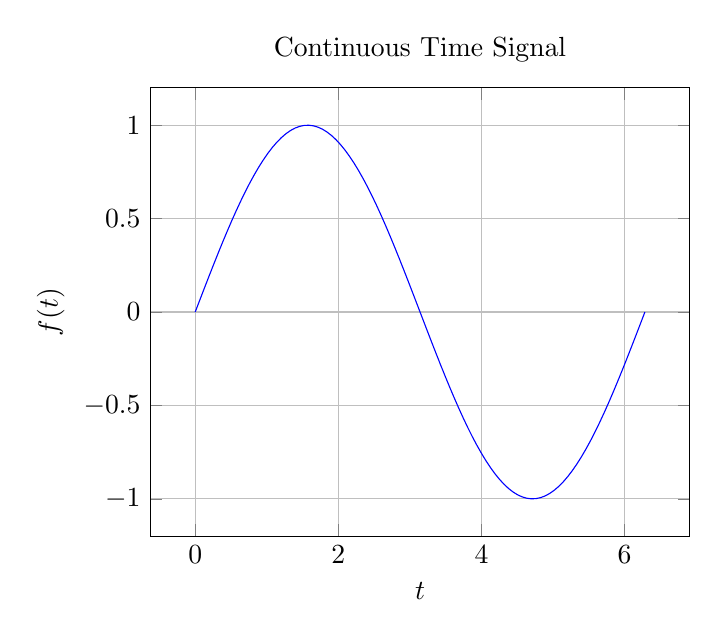
\begin{tikzpicture}
        \begin{axis}[
                xlabel={$t$},
                ylabel={$f(t)$},
                title={Continuous Time Signal},
                grid=both,
            ]
            \addplot[blue, domain=0:2*pi, samples=100] {sin(deg(x))};
        \end{axis}
    \end{tikzpicture}
    \caption{Continuous Time Signal}
    \label{CT signal}
\end{figure}

\begin{figure}[h]
    \centering
    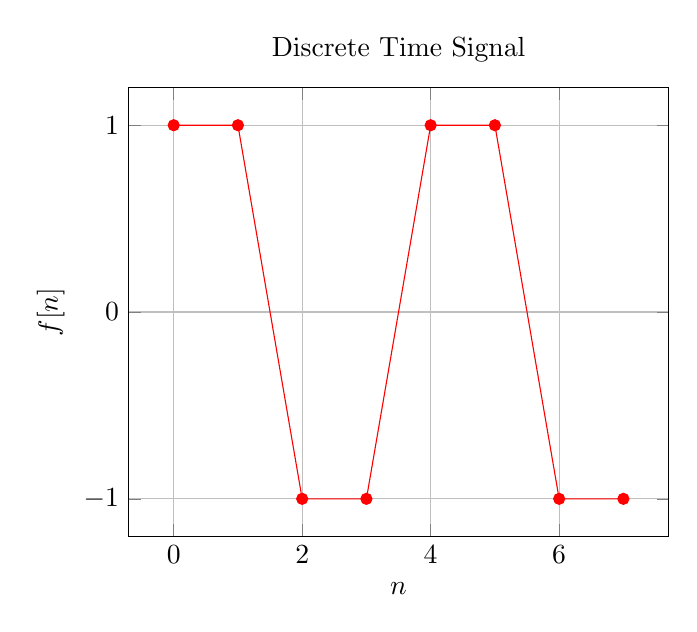
\begin{tikzpicture}
        \begin{axis}[
                xlabel={$n$},
                ylabel={$f[n]$},
                title={Discrete Time Signal},
                grid=both,
                ytick={-1,0,1},
            ]
            \addplot[red, mark=*] coordinates {
                    (0,1) (1,1) (2,-1) (3,-1) (4,1) (5,1) (6,-1) (7,-1)
                };
        \end{axis}
    \end{tikzpicture}
    \caption{Discrete Time Signal}
    \label{DT signal}
\end{figure}

In the most general terms, a systems transform inputs
to outputs. They're interconnections of subsystems.
Examples of systems include, topically, circuits.

Similarly to signals, there are continuous time systems
and discrete time systems. In a CT system, the input and
output are continuous. Conversely, DT systems have discrete
inputs and outputs.

\begin{figure}[h]
    \centering
    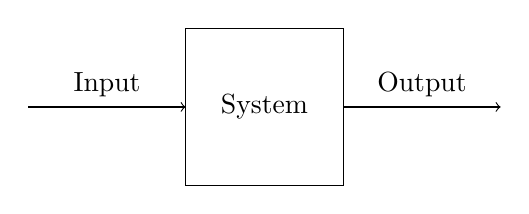
\begin{tikzpicture}
        \draw[->] (-3,0) -- (-1,0) node[midway, above] {Input};
        \draw (-1,-1) rectangle (1,1) node[midway] {System};
        \draw[->] (1,0) -- (3,0) node[midway, above] {Output};
    \end{tikzpicture}
    \caption{System Diagram}
    \label{System diagram}
\end{figure}

The astute reader will notice systems operate much like functions.
We use function notation to describe systems. For a CT system, we
write $y(t) = S(x(t))$ with parentheses to show it's CT. For DT,
we use brackets like $y[t] = S(x[t])$.

It's easy to imagine a system with continuous input and discrete output,
or vice versa. These are called samplers and reconstructors respectively.
We'll mostly be looking at linear time-invariant discrete systems, since they have the greatest
analogy to ECE.